\uuid{zVRx}
\exo7id{7140}
\titre{exo7 7140}
\auteur{megy}
\organisation{exo7}
\datecreate{2017-04-05}
\isIndication{true}
\isCorrection{true}
\chapitre{Géométrie affine euclidienne}
\sousChapitre{Géométrie affine euclidienne du plan}
\module{Géométrie}
\niveau{L2}
\difficulte{}

\contenu{
\texte{
Soit $ABCD$ un quadrilatère convexe inscriptible dont les diagonales sont perpendiculaires, et soit $O$ leur point d'intersection. Soit $H$ le projeté orthogonal de $O$ sur $[CD]$, et $I$ l'intersection de $(OH)$ avec $[AB]$. L'objectif est de montrer que $I$ est le milieu de $[AB]$. 


\begin{center}
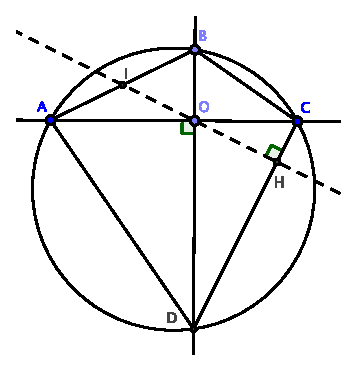
\includegraphics{../images/img007140-1}
\end{center}
}
\begin{enumerate}
    \item \question{Montrer qu'il est suffisant d'établir que $IO=IA$.}
\reponse{On rappelle que le milieu de l'hypoténuse d'un triangle rectangle est le centre de son cercle circonscrit (une autre façon de le dire est que l'hypoténuse est un diamètre du cercle circonscrit).

Si $IO=IA$, cela signifie que $I$ est sur la médiatrice de $[OA]$. D'autre part, $AOB$ est rectangle en $O$ et $I$ est par définition sur l'hypoténuse $[AB]$. Donc $I$ est  l'intersection de l'hypoténuse et d'une médiatrice d'un autre côté, c'est donc le milieu de l'hypoténuse par la propriété rappelée plus haut. Il est donc suffisant de montrer que $IO=IA$.}
    \item \question{Conclure.}
\reponse{Pour montrer que $IO=IA$, il suffit de montrer que $IOA$ est isocèle en $I$, c'est-à-dire que $(AI,AO)=(OA,OI)$. Or, on a :
\begin{align*}
(AI,AO)& = (AB,AC) \text{ (mêmes droites)}\\
&= (DB,DC) \text{ (car $ABCD$ est inscriptible}\\
&= (DO,DH) \text{ (mêmes droites)}\\
&= (DO,OH)+(OH,DH) \text{ (par Chasles)}\\
&= (DO,OH)+\pi/2 \text{ (par définition de $H$)}\\
&= (OB,OI)+\pi/2 \text{ (mêmes droites)}\\
&= (OB,OI) + (OA,OB) \text{ (car $(OA)\bot (OB)$ d'après l'énoncé)}\\
&= (OA,OI) \text{ (par Chasles)}
\end{align*}}
\indication{Où se trouve le centre du triangle circonscrit d'un triangle rectangle ?}
\end{enumerate}
}
